\documentclass[titlepage]{article}
\usepackage[draft=false, cachedir=minted_cache]{minted}
\usepackage{enumitem}
\usepackage{listings}
\usepackage{graphicx}
\graphicspath{ {./img/} }
\usepackage[margin=.5in]{geometry} %used to set the margins
\setcounter{secnumdepth}{0} %used to get rid of section numbers
\title{
    Project 3- Text Processing \\
    CSCI 230 T Th 11:10 am \\
    Compiler: g++ \\
    OS: Windows 10/WSL
    }

\author{Michael Morikawa}
\date{\today}


\begin{document}
\maketitle

\section{Notes}
\subsection{Status}
Both HuffmanCoding and Trie portion of the project are completed with no errors.
\subsection{Extra Credit}
Did the improved standard trie that gives the amount of times a word occurs.
\subsection{Design Decisions}
For the HuffmanCoding input, my program will only work with window style line endings. If
its not then it will not read a new line character. The solution for that is commented out in the code; to fix
it I would just need to add a newline after each call to getline and the remove the final newline character since it
will add an extra one.

For the trie I decided to ignore the numbers simply because the child array is much smaller. In order to include the numbers
while still using a lookup table as the child array it would have to be much larger since numbers are not right next to the lowercase letters in
the ascii table.


\newpage

\section{output}
\subsection{moneyOut.txt}
\lstinputlisting{../moneyOut.txt}
\subsection{Trie Output}
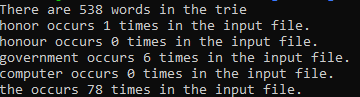
\includegraphics[]{trieOutput.png}

\newpage

\section{Source Code}
\subsection{main.cpp}
\inputminted{c++}{../../src/main.cpp}
\subsection{HuffmanNode.hpp}
\inputminted{c++}{../../include/HuffmanNode.hpp}
\subsection{HuffmanCoding.hpp}
\inputminted{c++}{../../include/HuffmanCoding.hpp}
\subsection{HuffmanCoding.cpp}
\inputminted{c++}{../../src/HuffmanCoding.cpp}
\subsection{Trie.hpp}
\inputminted{c++}{../../include/Trie.hpp}
\subsection{Trie.cpp}
\inputminted{c++}{../../src/Trie.cpp}


\end{document}